\documentclass{beamer}
\usetheme{metropolis}
\usepackage{graphicx}
\usepackage{amsmath}
\usepackage{hyperref}
\title{Digital Signal Processing: COSC360}
\author{Jordan Hanson}
\institute{Whittier College Department of Physics and Astronomy}

\begin{document}
\maketitle

\begin{frame}{Unit 1.1 Outline}
This lecture will cover:
\begin{enumerate}
\item \alert{Complex numbers 1: Arithmetic and some calculus (continuous and discete) ... see Chapter 30 of text}
\end{enumerate}
Next lectures will cover:
\begin{enumerate}
\item Complex numbers 2: The Fourier series and Fourier transform (continuous and discrete)
\item \textit{Time-permitting}: The Laplace transform (continuous and discrete)
\end{enumerate}
\end{frame}

\section{Complex numbers 1: theory and examples}

\begin{frame}{Complex numbers 1: Definition of a complex number}
A \alert{complex number} is an expression for which one term is proportional to $j = \sqrt{-1}$:
\begin{equation}
z = x + jy
\end{equation}
To call the \textit{complex unit} $j$ is the convention in electrical engineering, and in physics it is often called $i$. \\ \vspace{0.5cm}
Example of complex numbers: $(3+4j)$, $(x_1 + x_2 j)$.  Each number has a \textit{real} part and an \textit{imaginary} part.
\end{frame}

\begin{frame}{Complex numbers 1: Definition of a complex number}
Operations to learn:
\begin{enumerate}
\item Addition
\item Subtraction
\item Real part $\operatorname{Re}$ and $\operatorname{Im}$
\item Multiplication
\item Conjugation
\item Magnitude/Norm
\item Division
\end{enumerate}
Notations to learn:
\begin{enumerate}
\item Cartesian
\item Polar
\item Graphical
\end{enumerate}
\end{frame}

\begin{frame}{Complex numbers 1: Operations}
Addition follows the pattern of two-dimensional vectors:
\begin{align}
z_1 &= 3+4j \\
z_2 &= -2+5j \\
z_1 + z_2 &= 1+9j
\end{align} \\
Subtraction follows the pattern of two-dimensional vectors:
\begin{align}
z_1 &= 3+4j \\
z_2 &= -2+5j \\
z_1 - z_2 &= 5-1j
\end{align}
\end{frame}

\begin{frame}{Complex numbers 1: Operations}
\begin{figure}
\centering
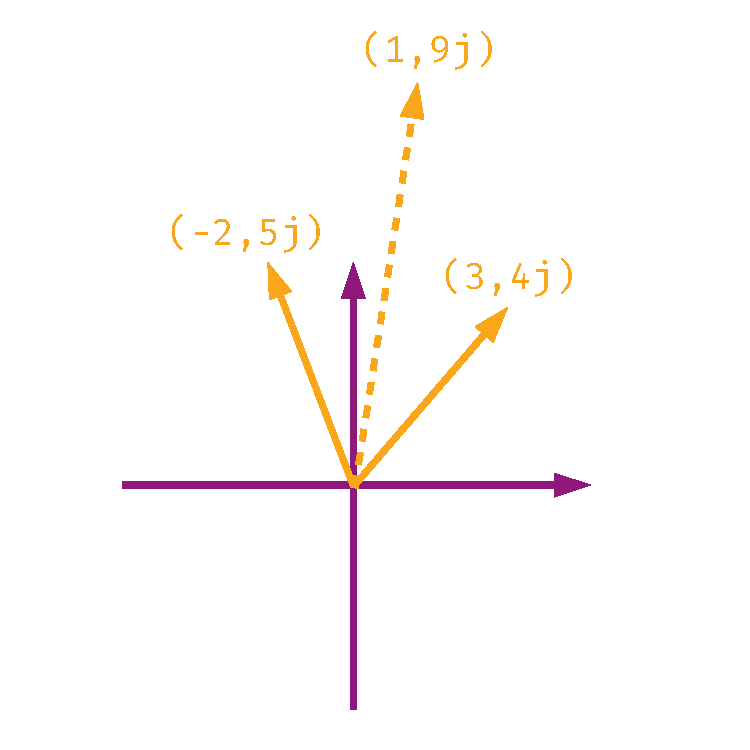
\includegraphics[width=0.45\textwidth]{figures/complexNumbers1.pdf}
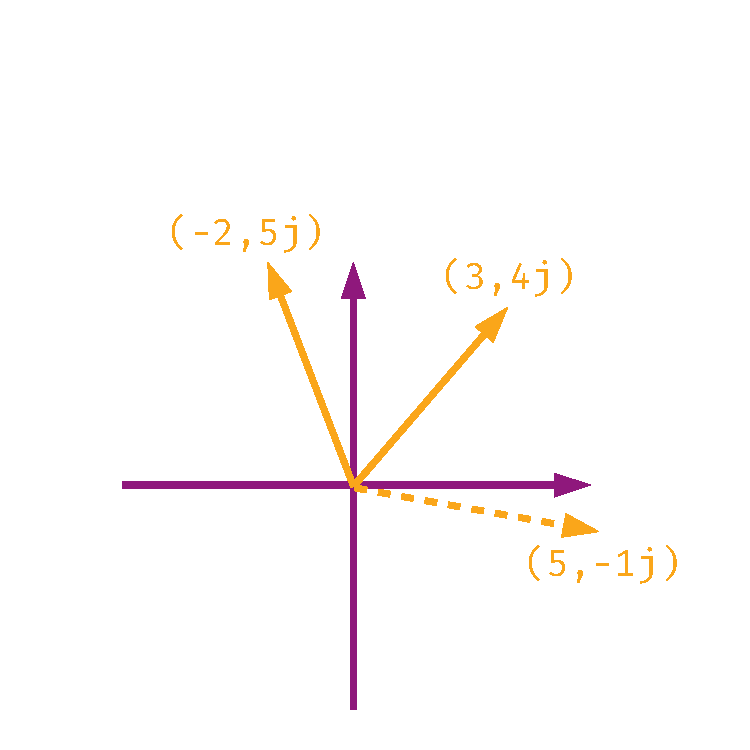
\includegraphics[width=0.45\textwidth]{figures/complexNumbers2.pdf}
\caption{\label{fig:complex1} Complex addition and subtraction follows the pattern of two-dimensional vectors. (Left): Addition of $z_1$ and $z_2$.  (Right): Subtraction of $z_1$ and $z_2$.}
\end{figure}
\end{frame}

\begin{frame}{Complex numbers 1: Operations}
We also have the $\operatorname{Re}$ and $\operatorname{Im}$ operations:
\begin{align}
z_1 &= 3+4j \\
\operatorname{Re}\lbrace z_1 \rbrace &= 3 \\
\operatorname{Im}\lbrace z_2 \rbrace &= 4
\end{align}
These are known as taking the \textit{real}-part and the \textit{imaginary}-part.  The original complex number can be recovered by adding real and imaginary parts together:
\begin{equation}
z_1 = \operatorname{Re}\lbrace z_1 \rbrace + j \operatorname{Im}\lbrace z_1 \rbrace
\end{equation} \\
When we add/subtract complex numbers, we combine the real parts and imaginary parts separately.
\end{frame}

\begin{frame}{Complex numbers 1: Operations}
Do these operators distribute?
\begin{align}
z_1 &= 3+4j \\
z_2 &= 5+12j \\
\operatorname{Re}\lbrace z_1+z_2 \rbrace &= 3+4j+5+12j = \operatorname{Re}\lbrace 8+16j \rbrace \\
\operatorname{Re}\lbrace z_1+z_2 \rbrace &= 8 = \operatorname{Re}\lbrace z_1 \rbrace + \operatorname{Re}\lbrace z_2 \rbrace \\
\operatorname{Im}\lbrace z_1+z_2 \rbrace &= 16 = \operatorname{Im}\lbrace z_1 \rbrace + \operatorname{Im}\lbrace z_2 \rbrace
\end{align}
They distribute because of the associativity of addition.
\end{frame}

\begin{frame}{Complex numbers 1: Operations}
\textit{Add or subtract, then simplify:}
\begin{enumerate}
\item $z_1 = 7+7j$, $z_2 = -6+3j$.  $z_1+z_2 = $
\item $z_1 = 2+2j$, $z_2 = 3-3j$.  $z_1-z_2 = $
\item $z_1 = 2x+7j$, $z_2 = 2+4xj$.  $z_1+z_2 = $
\end{enumerate}
Let $x=-1$ and $y=1$.  \textit{Evaluate the following expressions:}
\begin{enumerate}
\item $z_1 = x+yj$, $z_2 = y+xj$.  $z_1+z_2 = $
\item $z_1 = x^2+y^2j$, $z_2 = 2y^2+x^2j$.  $z_1-z_2 = $
\end{enumerate}
Draw a y-axis for the imaginary part, and an x-axis for the real part, and graph the prior two exercises.  Place points on the graph for $z_1$, $z_2$, and $z_1+z_2$.
\end{frame}

\begin{frame}{Complex numbers 1: Operations}
\textit{Multiplication: Recall that $j^2 = -1$.}
\begin{align}
z_1 &= x_1+jy_1 \\
z_2 &= x_2 + j y_2 \\
z_1 \times z_2 &= x_1 x_2 - y_1 y_2 + j (x_1 y_2 + x_2 y_1)
\end{align}
The cross-terms are straightforward, but remember the minus sign when multiplying the imaginary parts. \\ \vspace{0.5cm}
Examples:
\begin{enumerate}
\item $z_1 = 7+7j$, $z_2 = -6+3j$.  $z_1 \times z_2 = -42-21 + j(21-42) = -63-21j$.
\item $z_1 = 2+2j$, $z_2 = 2-2j$.  $z_1 \times z_2 = 8$.  Why no imaginary part?
\end{enumerate}
\end{frame}

\begin{frame}{Complex numbers 1: Operations}
Another similarity with two-dimensional vectors?
\begin{align}
z_1 &= 4-1j \label{eq:z1} \\
z_2 &= 1+4j \label{eq:z2} \\
z_1 \times z_2 &= 8 + 15j \neq 0
\end{align}
What would be the result if we were dealing with regular two-dimensional vectors?  Plot Eqs. \ref{eq:z1} and \ref{eq:z2} with the imaginary part as the y-coordinate and the real part as the x-coordinate.  Then draw a vector from the origin to the points.  Do you recall the properties of the \alert{dot-product} of two vectors?
\end{frame}

\begin{frame}{Complex numbers 1: Operations}
\begin{figure}
\centering
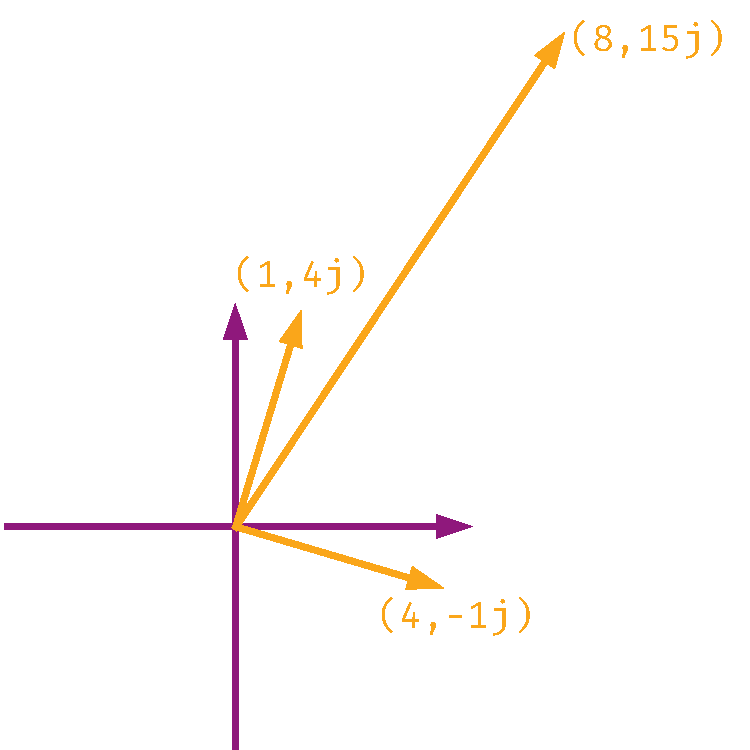
\includegraphics[width=0.45\textwidth]{figures/complexNumbers3.pdf}
\caption{\label{fig:complex2} Complex multiplication resembles the \textit{dot-product} for two-dimensional vectors, with key differences.}
\end{figure}
\end{frame}

\begin{frame}{Complex numbers 1: Operations}
Complex conjugation: change the sign of the imaginary part.
\begin{align}
z_1 &= 4-1j \\
z_1^* &= 4+1j \\
z_2 = &= 2x + 1j \\
z_2^* &= 2x - 1j
\end{align}
Is there a significance to $z_1 z_2^*$?  What about $z_1 z_1^*$?  What about $\sqrt{z_1 z_1^*}$? \\ \vspace{0.5cm}
What about the taking the complex conjugate of the following expression?
\begin{equation}
z = \frac{x_1 + jy_1}{x_2 + j y_2}
\end{equation}
\end{frame}

\begin{frame}{Complex numbers 1: Operations}
Multiply the denominator \textit{by the complex conjugate of the denominator.}
\begin{equation}
z = \frac{x_1 + jy_1}{x_2 + j y_2} \times \frac{x_1-j y_2}{x_2-j y_2}
\end{equation}
What happens?  The real and imaginary parts \textit{separate.}  Now prove that
\begin{equation}
z^* = \frac{x_1 - jy_1}{x_2 - j y_2}
\end{equation}
Let $z = (x_1+jy_1)(x_2+jy_2)$.  Prove that
\begin{equation}
z^* = (x_1 - jy_1)(x_2-jy_2)
\end{equation}
So it seems that complex conjugation boils down to finding all the imaginary units and making them negative...\textit{be careful about assuming this.}
\end{frame}

\begin{frame}{Complex numbers 1: Operations}
\begin{figure}
\centering
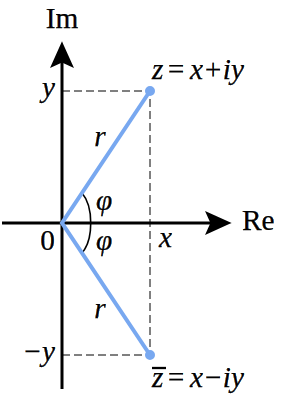
\includegraphics[width=0.4\textwidth]{figures/cc.png}
\caption{\label{fig:complex2a} Complex conjugation flips the location of the complex number if you draw the complex number as a coordinate pair.  Stay tuned for \alert{polar notation}.}
\end{figure}
\end{frame}

\begin{frame}{Complex numbers 1: Operations}
\small
Let $z = x+jy$.  Compute the following:
\begin{enumerate}
\item $zz^* = $
\item $\sqrt{zz^*} = $
\end{enumerate}
The second item on this list has a special name: the \textit{magnitude} or \textit{norm} of the complex number, $|z|$. \\ \vspace{0.5cm}
Compute the norm of the following complex numbers:
\begin{enumerate}
\item $2+2j$
\item $3+4j$
\end{enumerate}
Compute the norm.  Do either of these simplify?
\begin{enumerate}
\item $\sin(x)+j\cos(x)$
\item $\cos(x)+j\sin(x)$
\end{enumerate}
\end{frame}

\begin{frame}{Complex numbers 1: Operations}
Division of complex numbers: remember that there are multiple steps.
\begin{align}
z_1 &= x_1 + j y_1 \\
z_2 &= x_2 + j y_2 \\
\frac{z_2}{z_1} &= \frac{x_2 + j y_2}{x_1 + j y_1} \\
\frac{z_2}{z_1} &= \frac{z_2 z_1^*}{z_1z_1^*} = \frac{z_2 z_1^*}{|z_1|^2} \\
\frac{z_2}{z_1} &= \frac{\operatorname{Re} \lbrace{z_2 z_1^*}\rbrace}{|z_1|^2} + j \frac{\operatorname{Im} \lbrace{z_2 z_1^*}\rbrace}{|z_1|^2} \\
\frac{z_2}{z_1} &= \frac{x_1 x_2 + y_1 y_2}{x_1^2 + y_1^2} + j \frac{x_1 y_2 - x_2 y_1}{x_1^2 + y_1^2} \label{eq:div}
\end{align}
Using Eq. \ref{eq:div}, show that if $z_1 = z_2$, that $z_2/z_1 = 1$.
\end{frame}

\begin{frame}{Complex numbers 1: Operations}
Evaluate the divisions below:
\begin{enumerate}
\item $z_1 = 1+4j$, $z_2 = 2-2j$.  $z_2/z_1 = $
\item $z_1 = 1+1j$, $z_2 = -3-3j$.  $z_2/z_1 = $
\item $z_1 = 1+xj$, $z_2 = 1-xj$, and $x = 0.5$.  $z_2/z_1 = $
\end{enumerate}
What if $x$ had been imaginary?  Can you see a way to make the division infinity?
\end{frame}

\begin{frame}{Complex numbers 1: Polar Notation}
\begin{figure}
\centering
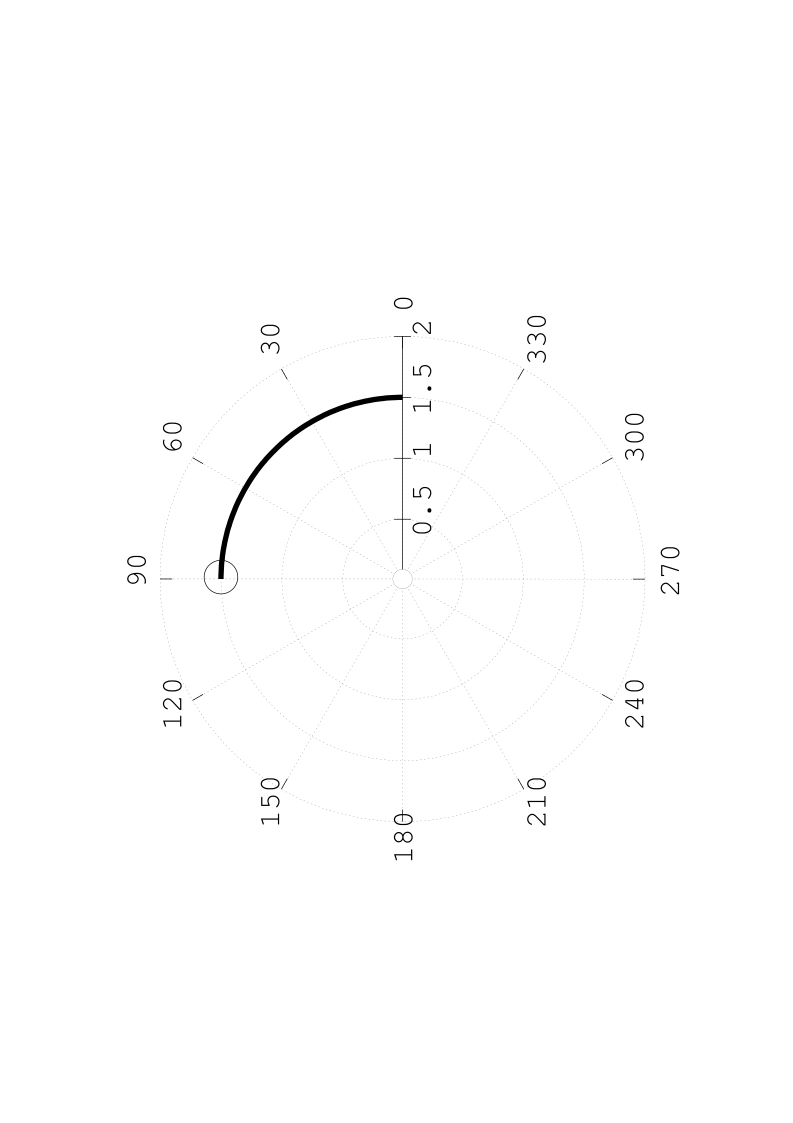
\includegraphics[width=0.5\textwidth,angle=270,trim=5cm 3cm 2cm 3cm]{figures/polar.png}
\caption{\label{fig:complex3} Polar coordinate systems rely on $(\rho,\phi)$ notation, rather than $(x,y)$ notation.}
\end{figure}
\end{frame}

\begin{frame}{Complex numbers 1: Polar Notation}
Polar notation for complex numbers: let $z = x+jy$.
\begin{align}
z &= r \exp(j\phi) \\
r &= |z| = \sqrt{x^2 + y^2} \\
\phi &= \tan^{-1}(y/x)
\end{align}
Useful for multiplication and division:
\begin{align}
z_1 &= r_1 \exp(j\phi_1) \\
z_2 &= r_2 \exp(j\phi_2) \\
z_1 \times z_2 &= r_1 r_2 \exp(j(\phi_1 + \phi_2)) \\
\frac{r_2}{r_1} &= \frac{r_2}{r_1} \exp(j(\phi_2 - \phi_1))
\end{align}
\end{frame}

\begin{frame}{Complex numbers 1: Polar Notation}
\small
Convert these complex numbers from Cartesian to polar form:
\begin{enumerate}
\item $z_1 = 5+13j$
\item $z_2 = 7-24j$
\item $z_3 = 20-21j$
\end{enumerate}
Divide:
\begin{enumerate}
\item $z_3/z_2$
\item $z_3/z_1$
\end{enumerate}
Multiply:
\begin{enumerate}
\item $z_1 \times z_2$
\item $z_1 \times z_1^*$
\end{enumerate}
\end{frame}

\begin{frame}{Complex numbers 1: Polar Notation}
How do you perform the complex conjugate in polar form? \textit{Change the sign of the phase angle.}
\begin{figure}
\centering
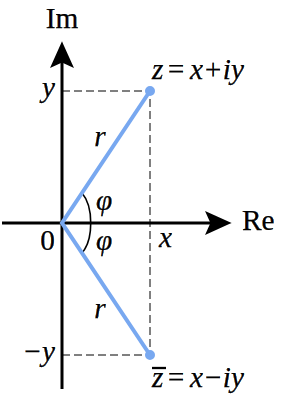
\includegraphics[width=0.3\textwidth]{figures/cc.png}
\caption{\label{fig:complex3a} Complex conjugation flips the sign of the angle.}
\end{figure}
\end{frame}

\begin{frame}{Complex numbers 1: Polar Notation}
Notice that the procedure for finding the modulus is evident in polar notation:
\begin{equation}
\sqrt{z_1 z_1^*} = \sqrt{r_1 r_1} \exp(j(\phi_1 - \phi_1)/2) = r_1
\end{equation}
Shouldn't we be saying $\pm r_1$?  How does the square root function work in the complex plane?\footnote{Complex fractional-power functions are outside the scope of the course, as it turns out, because it requires knowledge of the topic of \textit{branch cuts.}}
\end{frame}

\begin{frame}{Complex numbers 1: The complex plane}
\begin{figure}
\centering
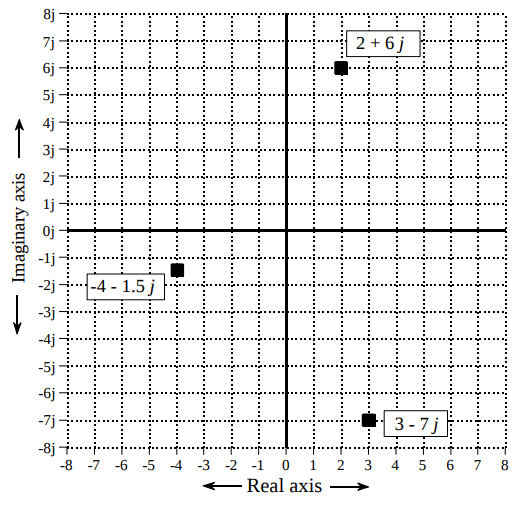
\includegraphics[width=0.5\textwidth]{figures/plane1.png}
\caption{\label{fig:complex4} The real and imaginary axes are an \textit{extension} of the real number line, allowing a broader representation of physical systems than just real numbers.  A prime example is AC circuits.}
\end{figure}
\end{frame}

\begin{frame}{Complex numbers 1: The complex plane}
\begin{figure}
\centering
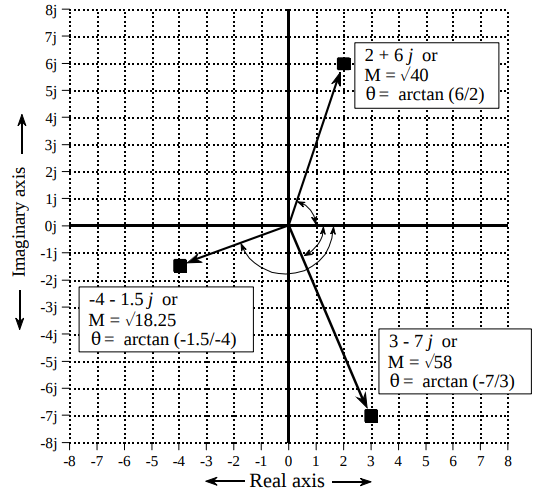
\includegraphics[width=0.5\textwidth]{figures/plane2.png}
\caption{\label{fig:complex5} Consider the complex plane in light of trigonometry.  Think of the magnitude of a complex number as the hypoteneuse of a right triangle.  Then, $\operatorname{Re}\lbrace z \rbrace = |z|\cos\phi$, and $\operatorname{Im}\lbrace z \rbrace = |z|\sin\phi$, and $r = |z| = \sqrt{x^2+y^2}$.}
\end{figure}
\end{frame}

\begin{frame}{Complex numbers 1: The complex plane}
\small
In the trigonometric picture:
\begin{equation}
z = |z| \cos\phi + j |z| \sin\phi
\end{equation}
Proof of polar-notation relationship:
\begin{align}
\exp(j\phi) &= \sum_{i=0}^{\infty} \frac{(j\phi)^n}{n!} = \sum_{i=0}^{\infty} \frac{j^n\phi^n}{n!} \\
\exp(j\phi) &= \sum_{even}^{\infty} \frac{j^n\phi^n}{n!} + \sum_{odd}^{\infty} \frac{j^n\phi^n}{n!} \\
\exp(j\phi) &= \sum_{i=0}^{\infty} (-1)^n \frac{\phi^{2n}}{(2n)!} + j\sum_{i=0}^{\infty} \frac{\phi^{2n+1}}{(2n+1)!} \\
\exp(j\phi) &= \cos\phi + j\sin\phi \\
|z|\exp(j\phi) &= |z| \cos\phi + j |z| \sin\phi = z
\end{align}
\end{frame}

\begin{frame}{Complex numbers 1: The complex plane}
Thus we have proven:
\begin{equation}
\boxed{ z = x+jy = r \exp(i\phi)
}
\end{equation}
Corollary (prove these):
\begin{align}
\cos(x) &= \frac{1}{2}\left(e^{ix} + e^{-ix}\right) \\
\sin(x) &= \frac{1}{2i}\left(e^{ix} - e^{-ix}\right)
\end{align}
Suppose we have now have a voltage signal
\begin{equation}
v_i(t) = A_i \cos(2\pi f_i t + \phi_i)
\end{equation}
We may write
\begin{equation}
v_i(t) = A_i \operatorname{Re}\lbrace \exp(j(2\pi f_i t + \phi_i)) \rbrace
\end{equation}
\end{frame}

\begin{frame}{Complex numbers 1: The complex plane}
What if we treat the signal as complex, but agree to take the real part at the end of our calculations?
\begin{equation}
v_i(t) \rightarrow A_i \exp(j(2\pi f_i t + \phi_i))
\end{equation}
As long as we take the real part of the right hand side, we'll have the original signal. \\ \vspace{0.5cm}
Now contemplate the addition of signals of the same frequency, but different amplitudes and phases.  Let $x_i = 2\pi ft+\phi_i$.  A signal comprised of $N$ sinusoids can be written
\begin{equation}
V_i(t) \rightarrow \sum_i^N a_i \exp(jx_i)
\end{equation}
\end{frame}

\begin{frame}{Complex numbers 1: The complex plane}
Remember that $x_i = 2\pi ft+\phi_i$.  The sum of two sinusoids in the complex plane can then be written\footnote{Notice that taking the real part distributes if the original signal is real.}
\begin{equation}
V(t) = a_1\exp(j x_1) + a_2\exp(j x_2)
\end{equation}
\begin{enumerate}
\item Compute $|V|^2 = V^*V$, and $\phi_2 - \phi_1 = \pi$, $\phi_2 - \phi_1 = 0$.
\item What is $\phi_V = \tan^{-1}(\operatorname{Im}\lbrace V \rbrace/\operatorname{Re}\lbrace V \rbrace)$ in each case?
\end{enumerate}
Why do these results make sense?  Thus, the complex numbers encapsulate the concepts of \textit{constructive} and \textit{destructive} interference.
\end{frame}

\begin{frame}{Complex numbers 1: The complex plane}
Treating sinusoids as rotation in the complex plane is a deep subject in physics.  It actually relates to some concepts in introductory physics: \url{https://www.youtube.com/watch?v=jxstE6A_CYQ} \\ \vspace{0.5cm}
What is the effect of multiplying by a complex number as follows:
\begin{equation}
V_i(t) \exp(j\phi') = ?
\end{equation}
What does this look like when graphed?
\end{frame}

\begin{frame}{Complex numbers 1: The complex plane}
\small
What if we continue to add terms, putting in carefully chosen phases and amplitudes?  We can represent \textit{any} periodic signal\footnote{We will return to this in Unit 1.2.}.  \\ \vspace{0.5cm}
This is known as the \textbf{\alert{Fourier series}}:
\begin{figure}
\centering
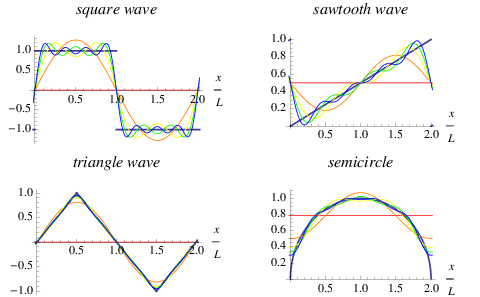
\includegraphics[width=0.5\textwidth]{figures/Fourier_Series.png}
\caption{\label{fig:fourier} The Fourier series representing four different periodic functions.}
\end{figure}
\end{frame}

%\section{Complex numbers 1: programming with Octave}

\begin{frame}{Complex numbers 1: programming with Octave}
Let's take the time to get octave installed on your systems.  Installation and tutorial are posted to Moodle: \url{https://cms.whittier.edu/mod/resource/view.php?id=507048} \\ \vspace{0.5cm}
Community support is broad and easily accessible: \url{https://wiki.octave.org/Category:Resources}
\end{frame}

\begin{frame}[fragile]{Complex numbers 1: programming with Octave}
Octave is a high-level \textit{scripting} programming language.  Although it is possible to write packages and compile code in octave, the most common application is executing a script that performs some analysis on digital data. \\
\begin{verbatim}
a = 1+1i;
b = conj(a);
a * b
\end{verbatim}
The result of this code should be 2.0.  Why?  We are defining a complex number in the first line, computing the complex conjugate, and multiplying them.
\end{frame}

\begin{frame}[fragile]{Complex numbers 1: programming with Octave}
Octave naturally handles vectors of numbers and matrices.  Let's define a vector of complex numbers. \\
\begin{verbatim}
a = [1 2 3 5 7 11];
size(a)
ans = 1   6
a = a';
size(a)
\end{verbatim}
The code in the fourth line \textit{transposes} the vector.  This means trading the rows for the columns of the vector.  What begins as a $1 \times 6$ vector (one row by six columns) ends as a $6 \times 1$ vector (six rows by one column).
\end{frame}

\begin{frame}[fragile]{Complex numbers 1: programming with Octave}
Operations are as expected, but we need special notation for vectoral calculations:
\begin{verbatim}
a = 2.0;
b = 4.0;
b/a
ans = 2
b = [4.0 4.0 4.0]
b/a
ans =
2   2   2
a./b
ans =
0.5   0.5   0.5
\end{verbatim}
\end{frame}

\begin{frame}[fragile]{Complex numbers 1: programming with Octave}
Placing a dot (.) before a standard operation indicates that the operation is to be carried out in a vectoral-sense.
\begin{verbatim}
t1 = [1 2 3 4 5 6 7 8 9 10];
t2 = t1+1;
t1.*t2
ans =
2   6   12   20   30   42   56   72   90   110
\end{verbatim}
\end{frame}

\begin{frame}[fragile]{Complex numbers 1: programming with Octave}
The colon operator (:) represents iteration in octave.  Consider three cases:  \\
\begin{verbatim}
fs = 1000.0;
t = [0.0:1/fs:10.0];
plot(t,sin(2.0 * pi * 3.0 .* t));
\end{verbatim}
Octave should produce a plot of a sine wave with a frequency of 3.0 Hz (if the time is in seconds).  How can you tell?
\end{frame}

\begin{frame}[fragile]{Complex numbers 1: programming with Octave}
Count the number of complete oscillations in 2.0 seconds.  Do you see 6.0 oscillations?  What is the significance of $f_s$ in the code?
\begin{verbatim}
fs = 1000.0;
t = [0.0:1/fs:10.0];
plot(t,sin(2.0 * pi * 3.0 .* t));
\end{verbatim}
The \alert{axis} command is useful for controlling the plotted region:
\begin{verbatim}
axis([0 2 -2 2]);
\end{verbatim}
\end{frame}

\begin{frame}[fragile]{Complex numbers 1: programming with Octave}
The colon operator (:) also refer to elements in a vector.
\begin{verbatim}
t(1)
ans =
0
t(2:5)
ans = 
0.001   0.002   0.003   0.004
t(:)
ans = 
(should be the whole vector)
t(1:end)
ans =
(should be the whole vector)
\end{verbatim}
\end{frame}

\begin{frame}[fragile]{Complex numbers 1: programming with Octave}
Now you know how to create vectors and plot them in octave.  Let's solve a few programming problems!  First, let's introduce the \alert{help} command.
\begin{verbatim}
help <command>
\end{verbatim}
Type the following commands
\begin{enumerate}
\item help plot
\item help :
\end{enumerate}
What is the purpose of the \textit{clear} and \textit{home} commands? \\ \vspace{0.5cm}
The key here is that if you are confused, the help command can boost your understanding of the correct usage.  Speaking of the colon command, how do we create matrices?
\end{frame}

\begin{frame}[fragile]{Complex numbers 1: programming with Octave}
\small
Create a matrix in octave in one of three ways:
\begin{enumerate}
\item \alert{Concatenate row vectors}
\item Concatenate colomn vectors
\item Write it straight away
\end{enumerate}
First, concatenation of row vectors:
\begin{verbatim}
a = [1:10];
b = [11:20];
A = [a; b];
display(A)
\end{verbatim}
The semi-colon also tells the $[]$ operators to concatenate vertically.  What is the size of the matrix?
\end{frame}

\begin{frame}[fragile]{Complex numbers 1: programming with Octave}
\small
Create a matrix in octave in one of three ways:
\begin{enumerate}
\item Concatenate row vectors
\item \alert{Concatenate colomn vectors}
\item Write it straight away
\end{enumerate}
First, concatenation of row vectors:
\begin{verbatim}
a = [1:10]';
b = [11:20]';
A = [a b];
display(A)
\end{verbatim}
The lack of the semi-colon tells the $[]$ operators to concatenate horizontally.  What is the size of the matrix?
\end{frame}

\begin{frame}[fragile]{Complex numbers 1: programming with Octave}
\small
Create a matrix in octave in one of three ways:
\begin{enumerate}
\item Concatenate row vectors
\item Concatenate colomn vectors
\item \alert{Write it straight away}
\end{enumerate}
First, concatenation of row vectors:
\begin{verbatim}
A = [[1 2]; [3 4];];
display(A)
\end{verbatim}
In this case, you can actually omit the internal concatenation operators.  Can you guess how to take the transpose of the matrix?
\end{frame}

\begin{frame}[fragile]{Complex numbers 1: programming with Octave}
\small
Create a matrix with complex numbers:
First, concatenation of row vectors, and take the transpose.  Do you notice something?
\begin{verbatim}
A = [[1 2i]; [3i 4];];
display(A)
\end{verbatim}
Try using the \textit{help} command on the transpose operator to sort out the issue.  Now look up the \textit{conj} command, and use it to take \textit{just the transpose} of the matrix, without conjugation.
\end{frame}

\begin{frame}[fragile]{Complex numbers 1: programming with Octave}
Two additional commands that are helpful for creating square ($N \times N$) matrices:
\begin{verbatim}
ones(N,M)
zeros(N,M)
\end{verbatim}
Create a $2 \times 2$ matrix and multiply it with a $2 \times 1$ vector.  \textit{Careful with the order; the matrix has to be on the left.} \\ \vspace{0.5cm}
You can imagine a matrix as an \textbf{\alert{operator}} that acts on a vector.  Example: two-dimensional rotation matrix (observe on board).
\begin{gather}
R(\theta) = \begin{bmatrix} \cos\theta & -\sin\theta \\ \sin\theta & \cos\theta \end{bmatrix} \label{eq:R}
\end{gather}
\end{frame}

\begin{frame}[fragile]{Complex numbers 1: programming with Octave}
Code the rotation matrix (Eq. \ref{eq:R}) for $\theta = \pi/4$, and also create three $2 \times 1$ column vectors.  Multiply them and display the results.  Plot them on the page and observe where they have moved. \\ \vspace{0.5cm}
\alert{Let's take the opportunity to share code on Moodle.}  \textbf{See the Rotation2D example in Unit1.} \\ \vspace{0.5cm}
Octave \textit{scripts} can be run within the octave environment.  I prefer octave-cli (\textit{command-line interface}), because it resembles a bash shell in linux systems.  The graphical user interface (octave-gui) can display folders, scripts, and the \textit{workspace.}  The workspace contains persistent variables.
\end{frame}

\section{Complex numbers 1: application to AC circuits}

\begin{frame}{Complex numbers 1: application to AC circuits}
\small
We touched on complex numbers in two contexts:
\begin{itemize}
\item Mathematical formalism
\item Programming octave
\end{itemize}
Now let's apply them to AC circuits.  Consider three circuit elements: the resistor, capacitor, and inductor.  They come with three symbols:
\begin{figure}
\centering
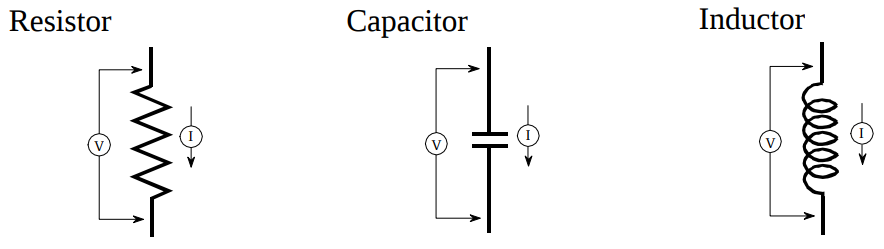
\includegraphics[width=0.75\textwidth]{figures/AC1.png}
\caption{\label{fig:AC1}  These three symbols can be combined in AC circuit diagrams to describe the flow of current and power.}
\end{figure}
\end{frame}

\begin{frame}{Complex numbers 1: application to AC circuits}
\small
We also need the concept of Ohm's law in the AC context:
\begin{equation}
V(\omega) = i(\omega) Z(\omega)
\end{equation}
The symbol $Z$ represents the \textit{complex resistance}, or \textit{impedance} of the circuit element.  Clearly, resistance can't be complex, but we think of the phase shift introduced to the current as being carried by a complex number.
\begin{align}
Z_R &= R + 0i \\
Z_C &= 0 + \frac{1}{j\omega C} \\
Z_L &= 0 + j \omega L
\end{align}
To \textit{prove} these equations, we'll need the \textit{Fourier transform}, and some circuit analysis (future lectures).  For now, think of them as just AC elements with (potentially) complex resistance.
\end{frame}

\begin{frame}{Complex numbers 1: application to AC circuits}
\small
Consider the circuit in Fig. \ref{fig:RLC1}.  If we think of $V_{in}$ as a sinudoidal signal, and $V_{out}$ as another sinusoidal signal, we can use complex numbers to compute what will happen at a given frequency $\omega$.
\begin{figure}
\centering
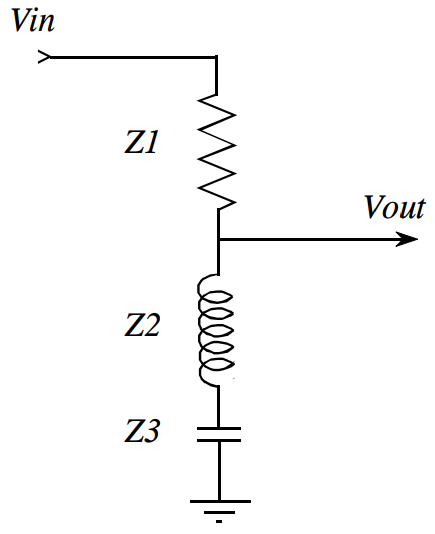
\includegraphics[width=0.3\textwidth]{figures/RLC1.png}
\caption{\label{fig:RLC1}  An example of an \textit{RLC} circuit.}
\end{figure}
\end{frame}

\begin{frame}{Complex numbers 1: application to AC circuits}
\small
\begin{figure}
\centering
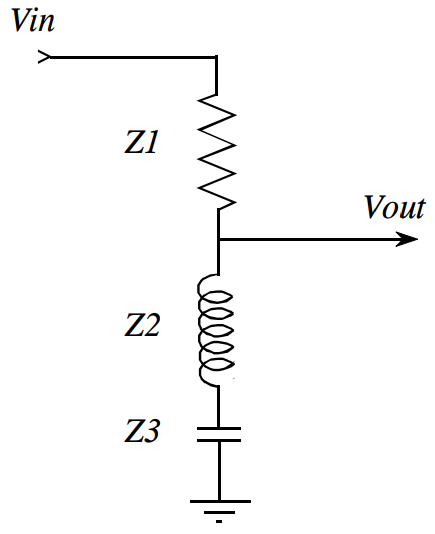
\includegraphics[width=0.3\textwidth]{figures/RLC1.png}
\caption{\label{fig:RLC2}  Using $V(\omega) = i(\omega) Z(\omega)$, we can solve for the ratio $V_{out}/V_{in}$.}
\end{figure}
Pretend that each AC element is some general element, and use Ohm's law to get the ratio $V_{out}/V_{in}$ (observe on board).
\end{frame}

\begin{frame}{Complex numbers 1: application to AC circuits}
We should find something like this:
\begin{align}
h(\omega) &= \frac{Z_2 + Z_3}{Z_1+Z_2+Z_3} \\
\omega_{LC}^{-2} &= LC \\
\tau &= RC \\
k^2 &= 1-\left(\frac{\omega}{\omega_{LC}}\right)^2 \\
h(\omega) &= \frac{k^4}{k^4+(\omega\tau)^2}-j \frac{k^2\omega\tau}{k^4+(\omega\tau)^2}
\end{align}
Notice that for $\omega = \omega_{LC}$, $k=0$.  What happens to $h(\omega)$ in that case?  What are the limits for $\omega \ll \omega_{LC}$ and $\omega \gg \omega_{LC}$?
\end{frame}

\begin{frame}{Complex numbers 1: application to AC circuits}
\begin{figure}
\centering
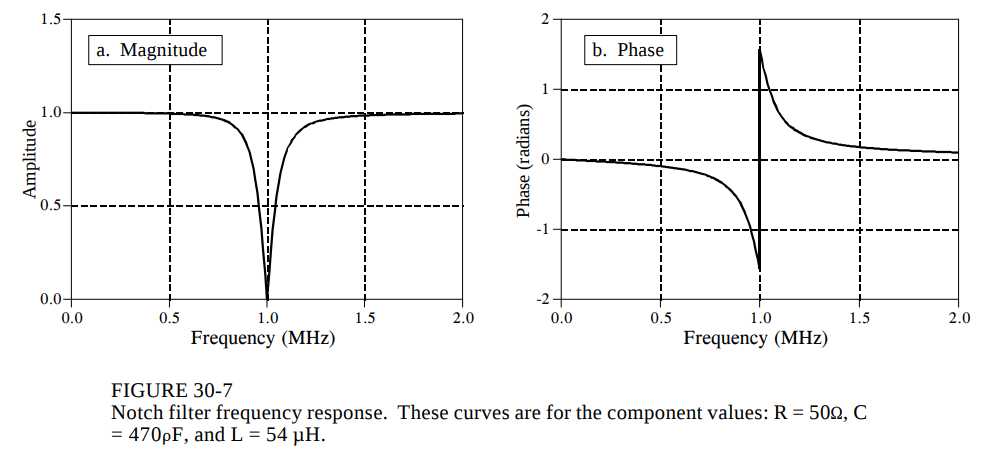
\includegraphics[width=0.95\textwidth]{figures/RLC2.png}
\caption{\label{fig:RLC3}  The magnitude and phase of the quantity $V_{out}/V_{in}$ are plotted versus frequerncy $f = \omega/(2\pi)$ for specific values of resistance, capacitance, and inductance.}
\end{figure}
\end{frame}

\begin{frame}{Complex numbers 1: application to AC circuits}
Today's octave application: write the script file \textit{RLC.m}, that reproduces Fig. \ref{fig:RLC3} for given values of R, L, and C.
\begin{itemize}
\item Write the script in a file entitled RLC.m
\item To run it, open octave-cli in the directory in which RLC.m is stored.  Type RLC, then hit enter.
\item We will cover plotting techniques on-the-fly, since plotting and markup could be an entire course.
\item Tweak the values of the AC elements and observe how your plot changes.  Why is this circuit one example of an \textit{RLC notch filter?}
\end{itemize}
\end{frame}

\section{Conclusion}

\begin{frame}{Unit 1.1 Outline}
Unit 1.1 covered:
\begin{enumerate}
\item \alert{Complex numbers 1: Arithmetic and some calculus (continuous and discete) ... see Chapter 30 of text}
\begin{itemize}
\item Complex number operations
\item Graphical knowledge of complex numbers
\item Octave coding
\item The RLC notch filter.
\end{itemize}
\end{enumerate}
Next lectures will cover:
\begin{enumerate}
\item Complex numbers 2: The Fourier series and Fourier transform (continuous and discrete)
\item \textit{Time-permitting}: The Laplace transform (continuous and discrete)
\end{enumerate}
\end{frame}

\end{document}
